\documentclass[12pt,a4paper]{scrreprt}

\usepackage{ucs}
\usepackage[utf8x]{inputenc}
\usepackage[T1]{fontenc}
\usepackage[ngerman]{babel}
\usepackage{graphicx}
\usepackage{listings}
\usepackage{color}

\usepackage{hyperref}

% Festlegung Art der Zitierung - Havardmethode: Abkuerzung Autor + Jahr
\bibliographystyle{}

% Literatur Datei
\bibliography{literatur}


\begin{document}

%verändert die Schriftart der Überschriften
\setkomafont{disposition}{\normalcolor\bfseries}

\begin{titlepage}

\centering

\title{Praxissemesterbericht \\  
\vspace{1cm} \large zu \\ 
\vspace{1cm}  Fuzzing mit American Fuzzy Lop \\
\vspace{0.5cm} bei der Firma \\
\vspace{0.5cm} Airbus DS Optronics GmbH \vspace{1.5cm}}


%\vspace{1.5cm}

\author{Andreas Eisele}

\vspace{1.5cm}

\date{\today{}, Aalen}
\maketitle
\end{titlepage}


\tableofcontents

\newpage
\renewcommand{\thesection}{\arabic{section}}


\chapter{Praxisstelle und Klausel}

\textbf{Airbus Defence \& Space Optronics GmbH}

\begin{minipage}{1\textwidth}

	Abteilung: \hspace{1cm} Softwareentwicklung \\
	Team: \hspace{1cm} ASSESS \\
	Adresse: 

\end{minipage}

\vspace{3cm}

\begin{minipage}{1\textwidth}

Hinweis zur Weitergabe bzw. Verwendung von ....

\end{minipage}



\newpage
\chapter{Eidesstattliche Erklärung}


\begin{minipage}{0.99\textwidth}

Hiermit erkläre ich, \textbf{Andreas Eisele}
dass ich die vorliegenden Angaben in diesem Bericht
zu meinen Tätigkeiten im Praxissemester bei
Airbus DS Optronics GmbH
wahrheitsgetreu und selbständig verfasst habe.
Weiterhin versichere ich, keine anderen als die angegebenen Quellen und Hilfsmittel benutzt zu haben, dass alle Ausführungen, die anderen Schriften wörtlich oder sinngemäß entnommen wurden, kenntlich gemacht sind und dass die Arbeit in gleicher oder ähnlicher Fassung noch nicht Bestandteil einer Studien- oder
Prüfungsleistung war. (Soweit mir bekannt!)

\vspace{2cm}

\end{minipage}

\begin{minipage}{0.99\textwidth}

Ort,  Datum \hspace{3cm} Unterschrift (Student)

\end{minipage}

%---------------------------------------------------------------

\vspace{3cm}

\begin{minipage}{0.99\textwidth}

Bestätigung der inhaltlichen Richtigkeit:
Der vorliegende Bericht wurde durch den zuständigen Betreuer
\textbf{Michael Adam} korrekturgelesen und auf inhaltliche Korrektheit geprüft.

\vspace{2cm}

\end{minipage}


\begin{minipage}{0.99\textwidth}

Ort, Datum \hspace{3cm} Unterschrift (Betreuer)

\end{minipage}


\newpage
\chapter{Kurzfassung}
Im Rahmen dieser Arbeit wird folgendes vorgestellt ........


\newpage
\chapter{ Motivation und Ziel der Arbeit  }

\section{Motivation}

Das testen von Software ist einer der wichtigsten Entwicklungsschritte eines jeden Software-Entwicklungsmodells. 

Oftmals ist die Testphase einem erhöhten Zeitdruck ausgesetzt und demzufolge wird sie nicht selten in einem deutlich verkürzten Rahmen durchgeführt.
Das hat zur Folge, dass sehr oft "Bugs" in Software enthalten sind, die mit entsprechenden Anstrengungen beziehungsweise einem guten Testverfahren gefunden werden können. Dabei ist der Aspekt ein qualitativ gutes Produkt zu liefern genauso wichtig, wie der Prävention vor Schwachstellen, die von Cyber-Kriminellen ausgenutzt werden könnten. 

Mit Fuzzer Programmen hat sich eine Testmethode etabliert, die weitaus mehr Testfälle abdecken kann und dies in deutlich kürzerer Zeit als das mit herkömmlichen Testverfahren möglich ist.
Insbesondere die jüngsten Fuzzer Tools sind oft vielseitig einsatzfähig und werden immer attraktiver in der Handhabung.


\section{Ziel der Arbeit}

Mit diesem Pilotprojekt soll getestet werden, ob sich einer der heutzutage populärsten Fuzzer zum einen gut in den Testprozess einbinden lässt und zum anderen ob die Ergebnisse der Testläufe auch den Erwartungen entsprechen.

Zudem soll die Frage geklärt werden, wie portabel der Fuzzer auf unterschiedliche Zielsysteme ist.


\chapter{Vorgehen}



\newpage
\chapter{Grundlagen} 

\section{Fuzzing}
Fuzzing auch als "Robustheits - Prüfung" bekannt, ist eine Methode um Software auf Stabilität und Schwachstellen zu testen. 

Im Vergleich zu Unit-Tests, bietet Fuzzing ein weitaus größeres Spektrum an generierten Zufallsdaten, welche auf die Zielschnittstellen ausgeführt werden.
Zudem werden die Daten nicht abhängig von dem verantwortlichen Entwickler bestimmt, sondern stellen tatslächliche Zufallsdaten oder Mutationen dar. Das grundlegende Prinzip von Fuzzing ist damit das "beschießen" der Zielsoftware mit generierten Zufallsdaten und so zu überprüfen, ob sich das Programm unerwartet verhält und dadurch eine Schwachstelle afgetreten ist.

Als unerwartetes Verhalten ist in der Regel das hängen oder abstürzen einer Software gemeint. Diese "Bugs" haben als Ursache oft Speicherleks, welche häufig in den Sprachen C und C++ auftreten, da diese dort nicht bereits automatisiert abgefangen werden. Die Schwachstellen, welche durch so einen Bug auftreten können, sind oft auch Ziel von Kriminellen die insbesondere bei sensibler Software wie Kommunikationsprogrammen hier schaden anrichten können.

Das erste mal wurde der Begriff Fuzzing und diese Methode zu testen von Barton Miller und seinen Studenten an der University of Wisconsin-Madison 1989 entwickelt.
Viele Jahre konnte sich Fuzzing für den breiten Gebrauch nicht etablieren. Aufgrund von sehr aufwendigen Anpassungen die notwendig waren um die damaligen Fuzzer-Tools auf die entsprechende Zielsoftware zuzuschneiden waren diese für die Testphase schlicht zu kostenintensiv. 

In den letzten Jahren hat durch die Entwicklung effizienterer Tools das Thema Fuzzing eine deutlich höhere Verbreitung erfahren. Besonders einer dieser Fuzzing-Programme wird im Rahmen dieser Arbeit behandelt.   

\newpage

\section{American Fuzzy Lop}
AFL wurde 2014 von Michal Zalewski entwickelt. Im Vergleich zu anderen verfügbaren Fuzzing-Tools unterscheidet sich American Fuzzy Lop maßgeblich, durch dessen neuen Ansatz mit einem genetischen instrumenten-geführten Algorithmus. Die Resultate durch den Einsatz dieses Tools haben sich signifikant verbessert und so zu dessen Bekanntheit geführt. 
Dieses Fuzzer-Programm ist in der Lage sowohl Black-Box als auch White-Box Tests durchzuführen und ist als freie Open-Source-Software unter der Apache Version 2 Lizenz verfügbar. 

Es zeichnet sich insbesondere durch die Instrumentierung während des Kompilierprozesses aus und erreicht dadurch eine sehr hohe Pfadabdeckung des Ziels. Indem Instruktionen in den Assembler-Code geschrieben werden, ist AFL in der Lage auf Veränderungen die im Ziel-Programm ausgelöst werden zu erfassen und darauf zu reagieren.
Eine weitere Besonderheit sind die Mutationen auf die Sample-Dateien. Um überhaupt fuzzen zu können muss mindestens eine minimale valide Datei vorliegen, welche von dem zu testenden Porgramm verarbeitet wird. Diese Dateien werden in einer Queue gespeichert und fortlaufend modifiziert oder verworfen. Wenn eine dieser Veränderungen einen neuen Programzustand verursacht wird diese Datei in die Queue mit aufgenommen.

Dieser Prozess wird immer wieder wiederholt, bis alle möglichen Programpfade mit den mutierten Dateien in der Zielsoftware durchlaufen wurden.



\begin{figure}[htbp] 
  \centering
     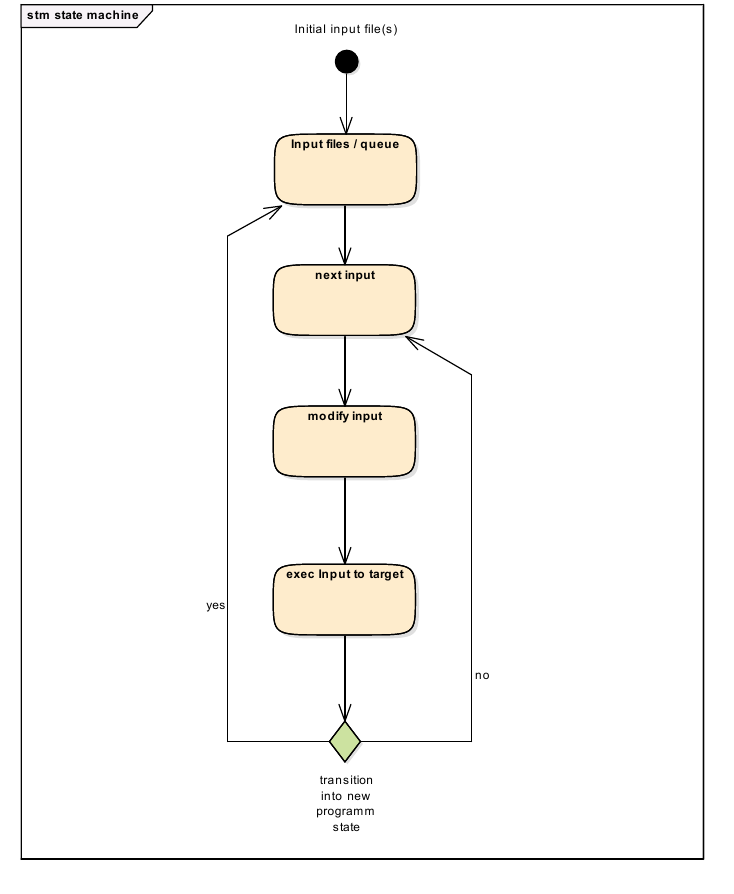
\includegraphics[width=0.75\textwidth]{state_machine.png}
  \caption{AFL State-Machine}
  \label{fig:Bild0}
\end{figure}




\subsection{Welche Software kann mit AFL getestet werden?}
AFL wurde in erster Linie für Programme entworfen, die Dateien verarbeiten oder über Stdin Eingaben erhalten. 

\newpage
\subsection{Instrumentierung}	
sjfnl

\subsection{Erfassen neuer Programzustände}

\subsection{Mutation}

\subsection{Fuzzing Session}

\subsection{Evaluation}

\section{mehr Grundlagen ......}

%-----------------------------------------------------------------

\newpage
\chapter{Zielsoftware (System - Stack)}
Der System Stack ist die softwareseitige Lösung für die Kommunikation zwischen verschiedenen Aufnahmegeräten.

Ein Master-Stack kann mit mehreren Slave-Stack`s kommunizieren. Der Stack ist in mehrere Schichten aufgeteilt die über Schnittstellen miteinander verbunden sind. Im Einsatz ruft ein Device seinen Stack beziehungsweise die oberste Schicht auf um Daten zu übertragen und der Stack wiederum über seine unterste Schicht ein entsprechendes IO\_Device um die Daten zu übertragen.


\section{Aufteilung des Ziels in Schichten}

Wie in dem Abschnitt ....... angesprochen, ist Software die von sich aus nicht schon Dateien oder Stdin-Eingaben verarbeitet daraufhin anzupassen.

Im Falle des System-Stack wurden die einzelnen Schichten für sich oder teils mit darüber- oder darunterligenden Schichten geprüft. 



\newpage
\section{Mitschneiden von Programmdaten}

\begin{figure}[htbp] 
  \centering
     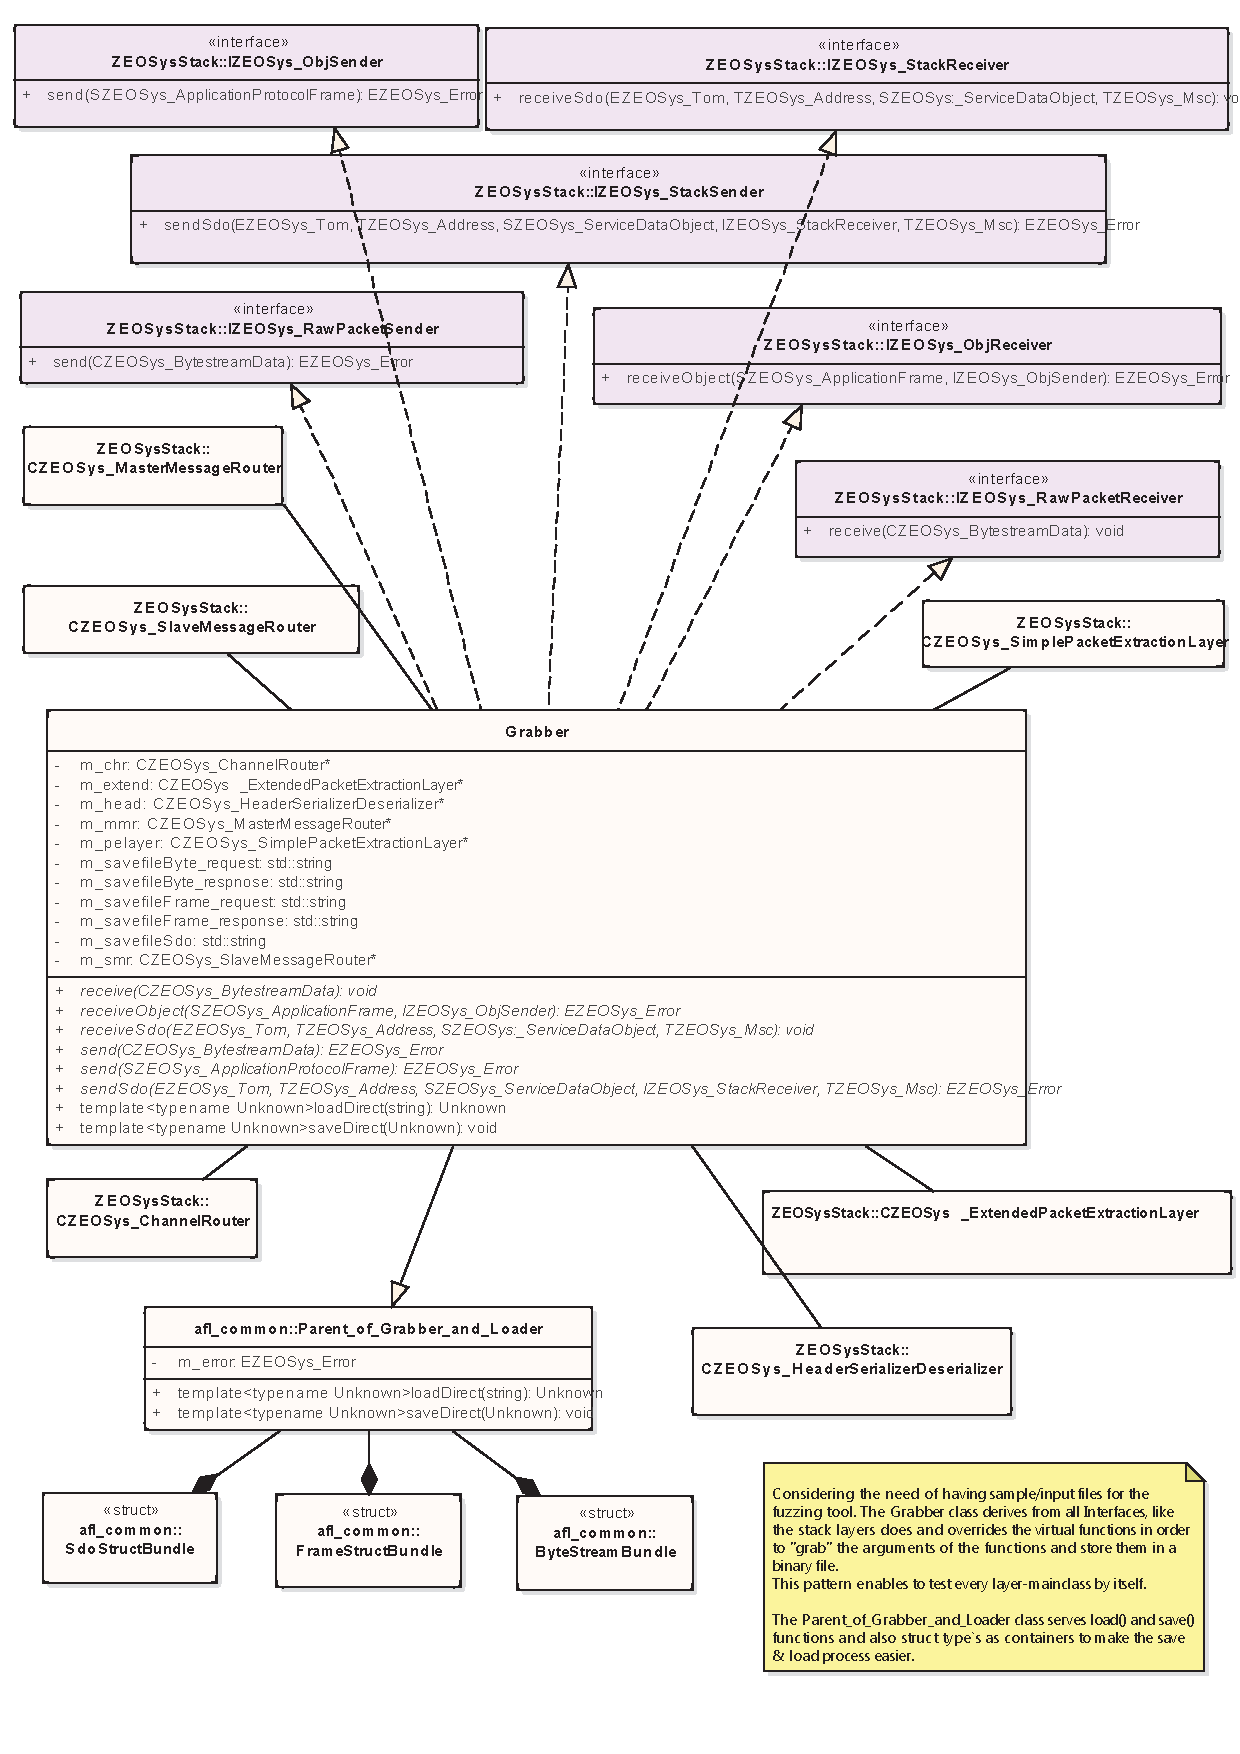
\includegraphics[width=1.0\textwidth]{generate.pdf}
  \caption{Grabber Klasse}
  \label{fig:Bild1}
\end{figure}


\begin{figure}[htbp] 
  \centering
     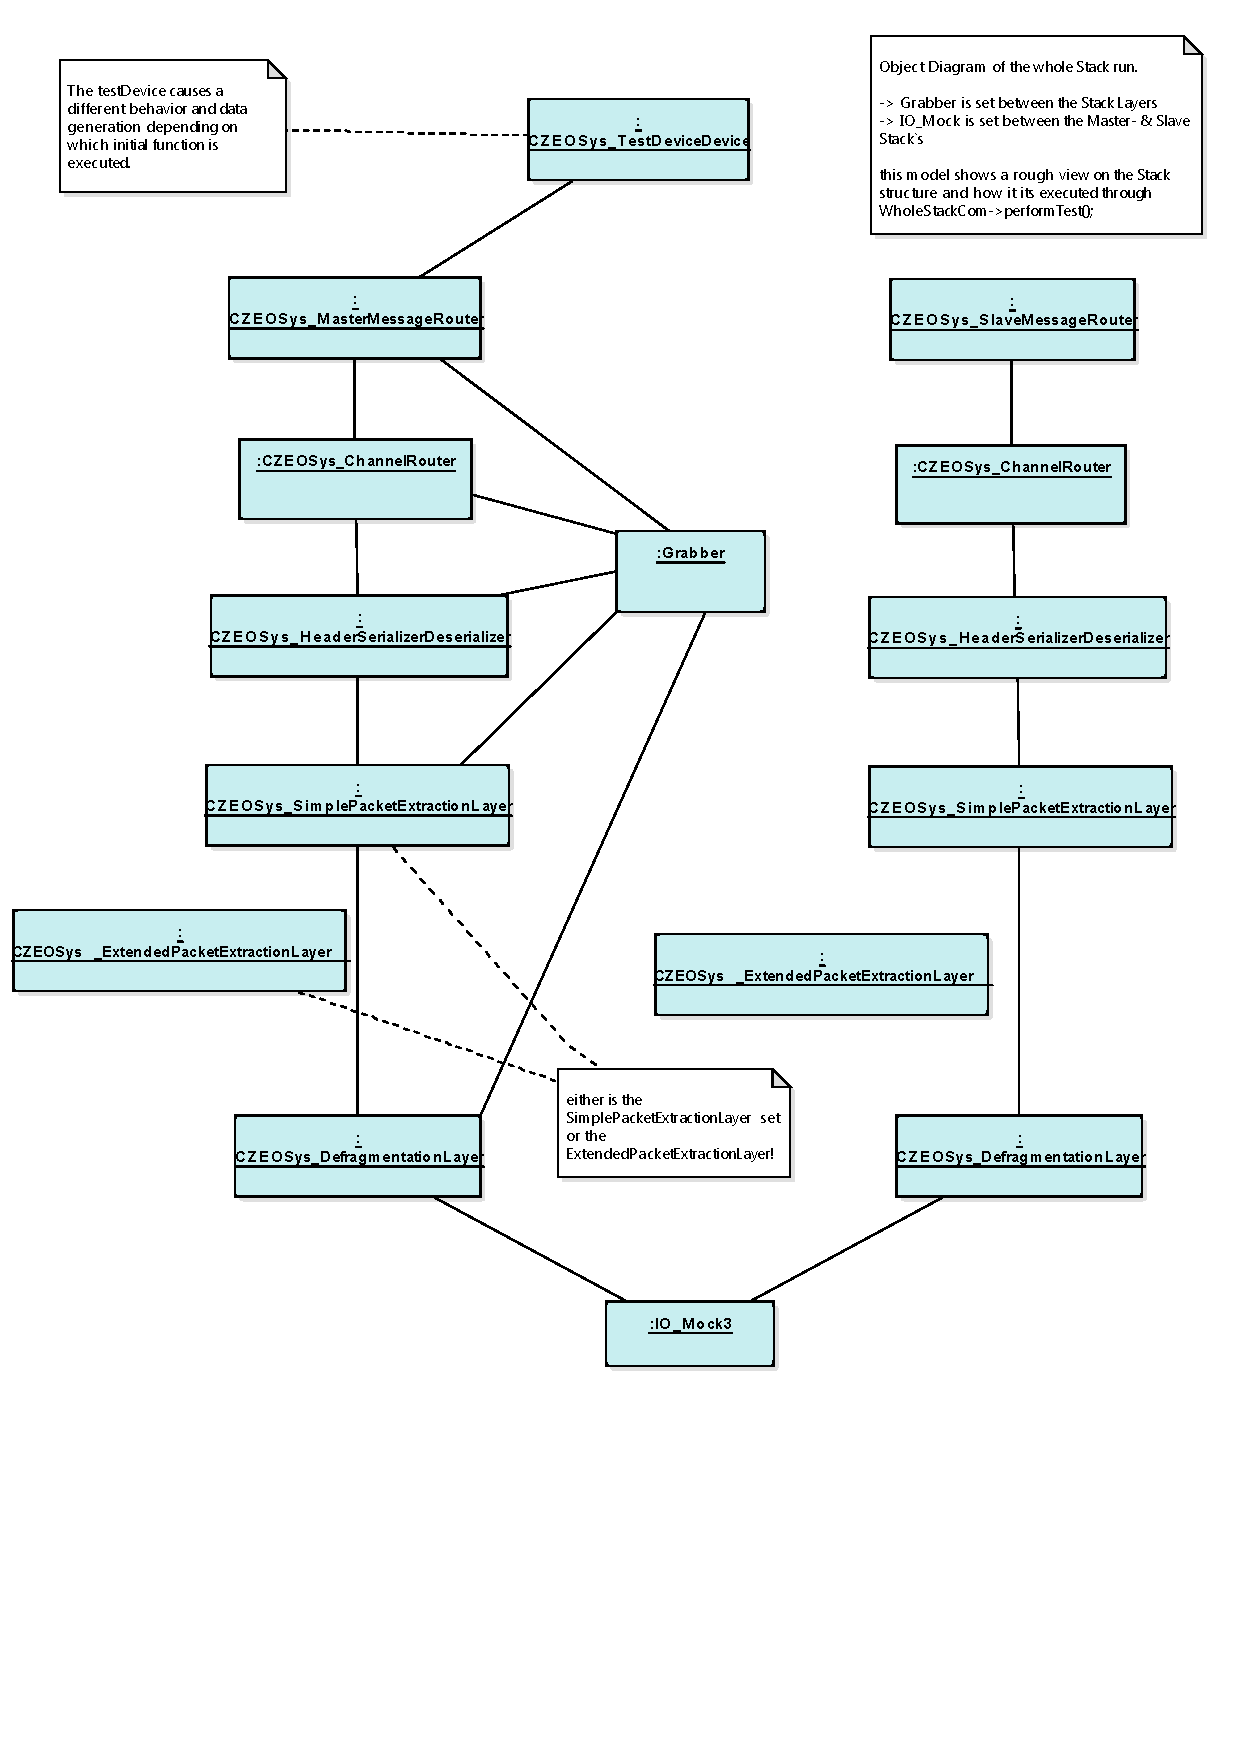
\includegraphics[width=1.0\textwidth]{object_diagramm.pdf}
  \caption{Einbettung Grabber}
  \label{fig:Bild2}
\end{figure}

\newpage
\section{Testumgebungen anlegen}

\begin{figure}[htbp] 
  \centering
     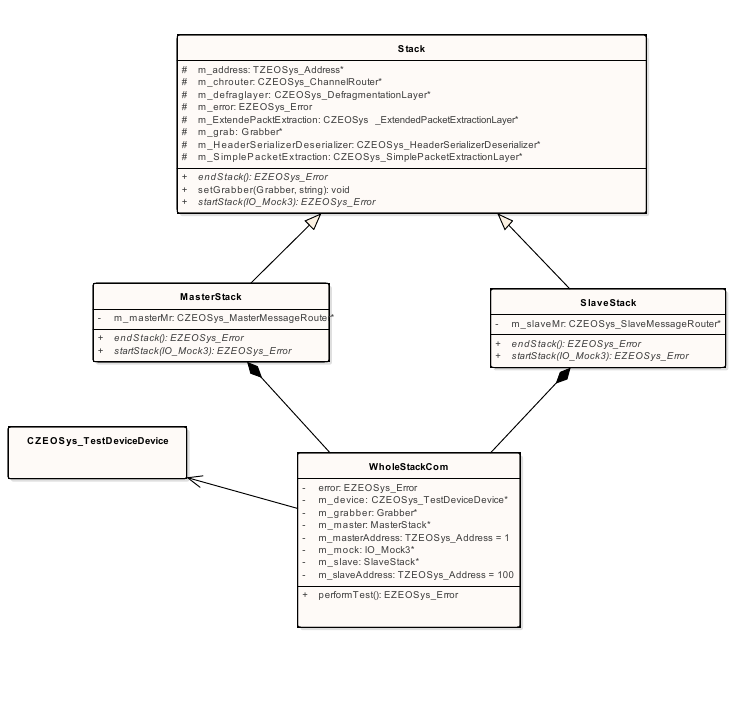
\includegraphics[width=1.0\textwidth]{stack.png}
  \caption{Stack Aufbau}
  \label{fig:Bild3}
\end{figure}


\begin{figure}[htbp] 
  \centering
     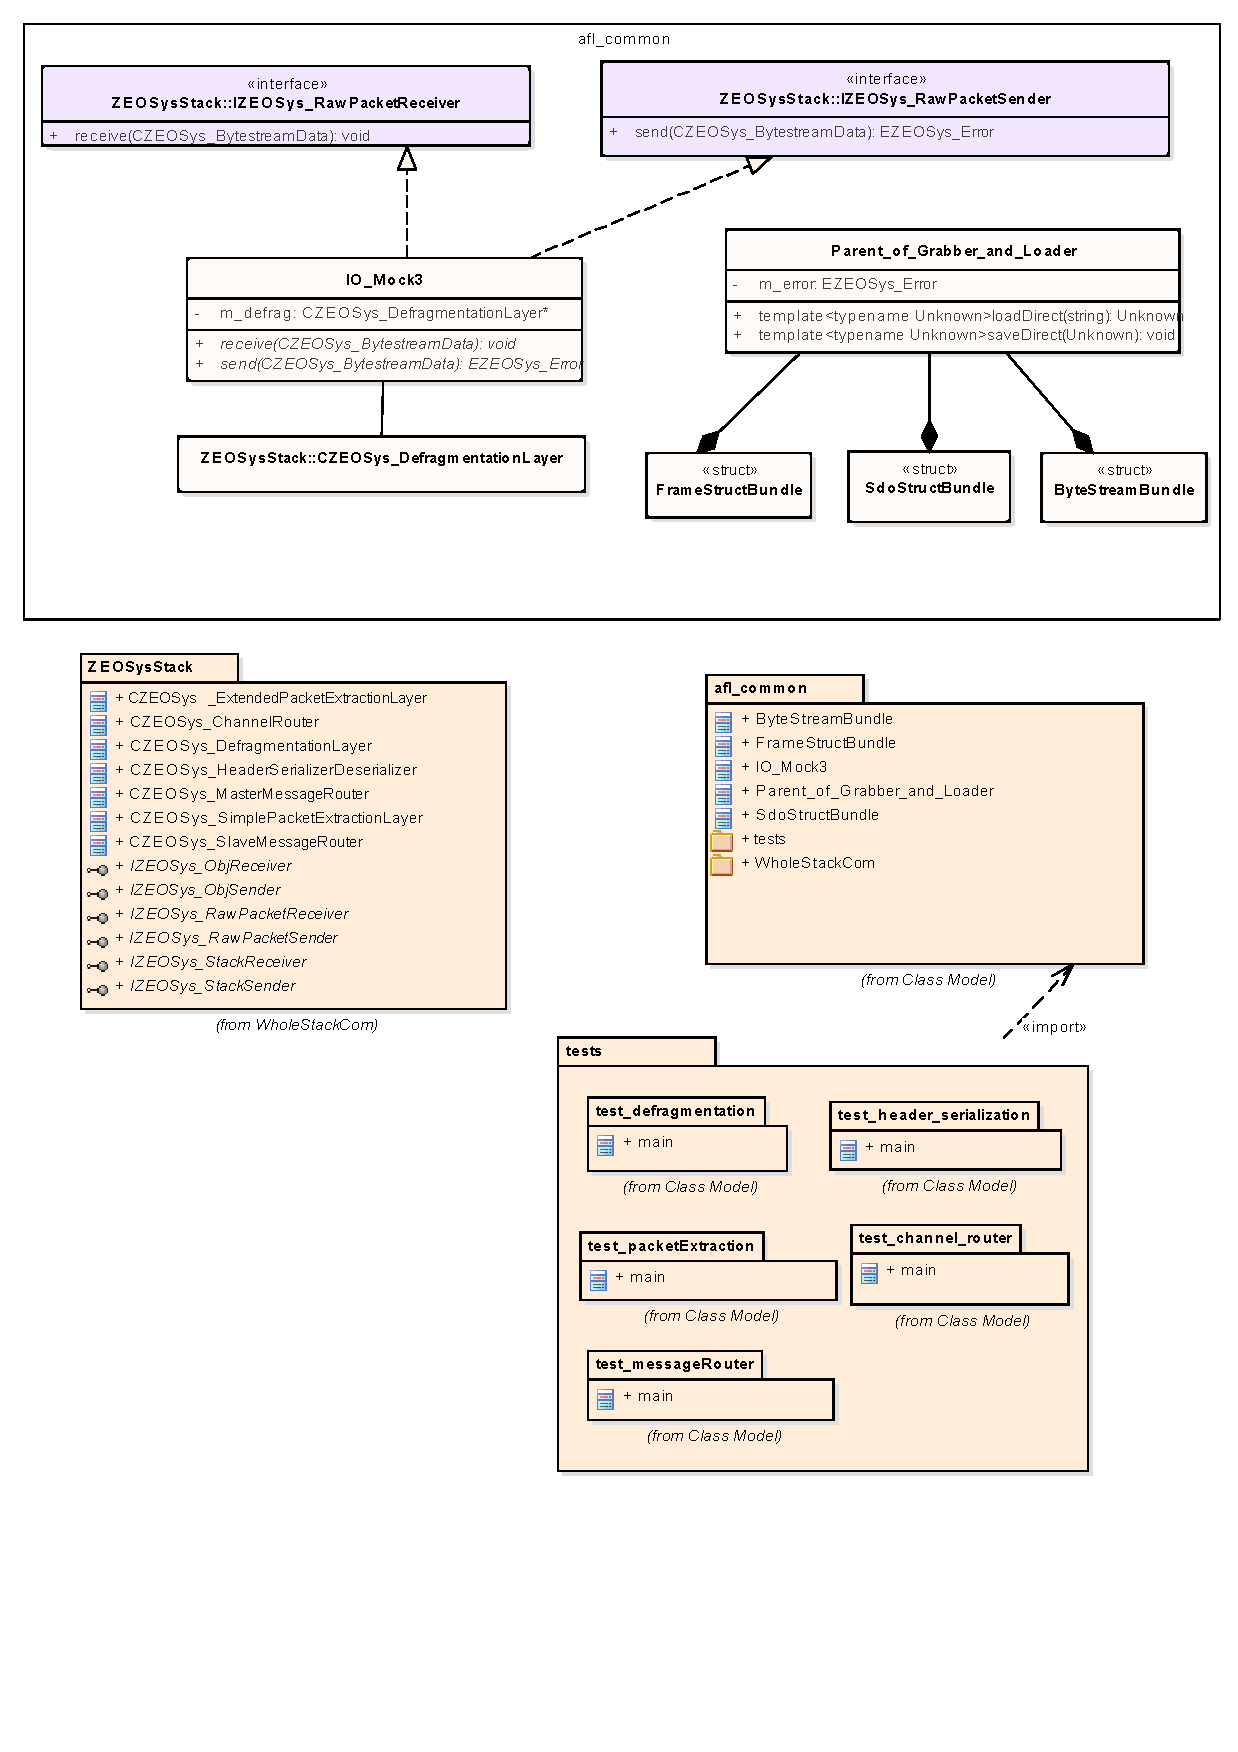
\includegraphics[width=1.0\textwidth]{afl_common.pdf}
  \caption{Paketmodell Testumgebung}
  \label{fig:Bild4}
\end{figure}


% Using typewriter font: \ttfamily inside \lstset
%\begin{frame}

%\lstset{language=C++,
%                basicstyle=\ttfamily,
%                keywordstyle=\color{blue}\ttfamily,
%                stringstyle=\color{red}\ttfamily,
%                commentstyle=\color{green}\ttfamily,
%                morecomment=[l][\color{magenta}]{\#}
%}
%\begin{lstlisting}
%    #include<stdio.h>
%    #include<iostream>
%    // A comment
%    int main(void)
%    {
%    printf("Hello World\n");
%    return 0;
%    }
%\end{lstlisting}
%\end{frame}


\newpage
\subsection{Auswertung der Testdaten}


\newpage
\section{Probleme und Lösungen}

\section{Fazit und Zusammenfassung}

\section{Quellen}

% https://fuzzing-project.org/tutorial1.html
% http://lcamtuf.coredump.cx/afl/README.txt
% http://lcamtuf.coredump.cx/afl/technical_details.txt
% https://steemit.com/security/@burnin/finding-software- vulnerabilities-by-fuzzing-with-american-fuzzy-lop
%https://en.wikipedia.org/wiki/Fuzzing

\section{Abbildungsverzeichnis}
\listoffigures	
	


\end{document}